%
% $RCSfile: functionality_in_detail.tex,v $
%
% Copyright (C) 2002-2008. Christian Heller.
%
% Permission is granted to copy, distribute and/or modify this document
% under the terms of the GNU Free Documentation License, Version 1.1 or
% any later version published by the Free Software Foundation; with no
% Invariant Sections, with no Front-Cover Texts and with no Back-Cover
% Texts. A copy of the license is included in the section entitled
% "GNU Free Documentation License".
%
% http://www.cybop.net
% - Cybernetics Oriented Programming -
%
% http://www.resmedicinae.org
% - Information in Medicine -
%
% Version: $Revision: 1.1 $ $Date: 2008-08-19 20:41:06 $ $Author: christian $
% Authors: Christian Heller <christian.heller@tuxtax.de>
%

\section{Functionality in Detail}
\label{functionality_in_detail_heading}
\index{CYBOI Functionality}
\index{CYBOI Part Dependencies}
\index{CYBOI Control Flow}

CYBOI's architecture is based on three main parts, as introduced by figure
\ref{architecture_figure} before: \emph{Controller}, \emph{Applicator} and
\emph{Memoriser}. (The \emph{Globals} package is neglectable for the following
explanations, since it contains static constants and variables that are
\emph{omnipresent}.) They appear again in figure \ref{dependencies_figure}
which shows the \emph{Dependencies} between them. Additionally, the
\emph{Controller} modules and their \emph{Control Flow} is illustrated.
Starting from the \emph{cyboi} module, the following subsections will
demonstrate how CYBOI functions internally, along the flow of control touching
the modules: \emph{manager}, \emph{checker} and \emph{handler}. After that, the
execution of operations in the \emph{Applicator} as well as the creation and
transition of data in the \emph{Memoriser} are described.

\begin{figure}[ht]
    \begin{center}
        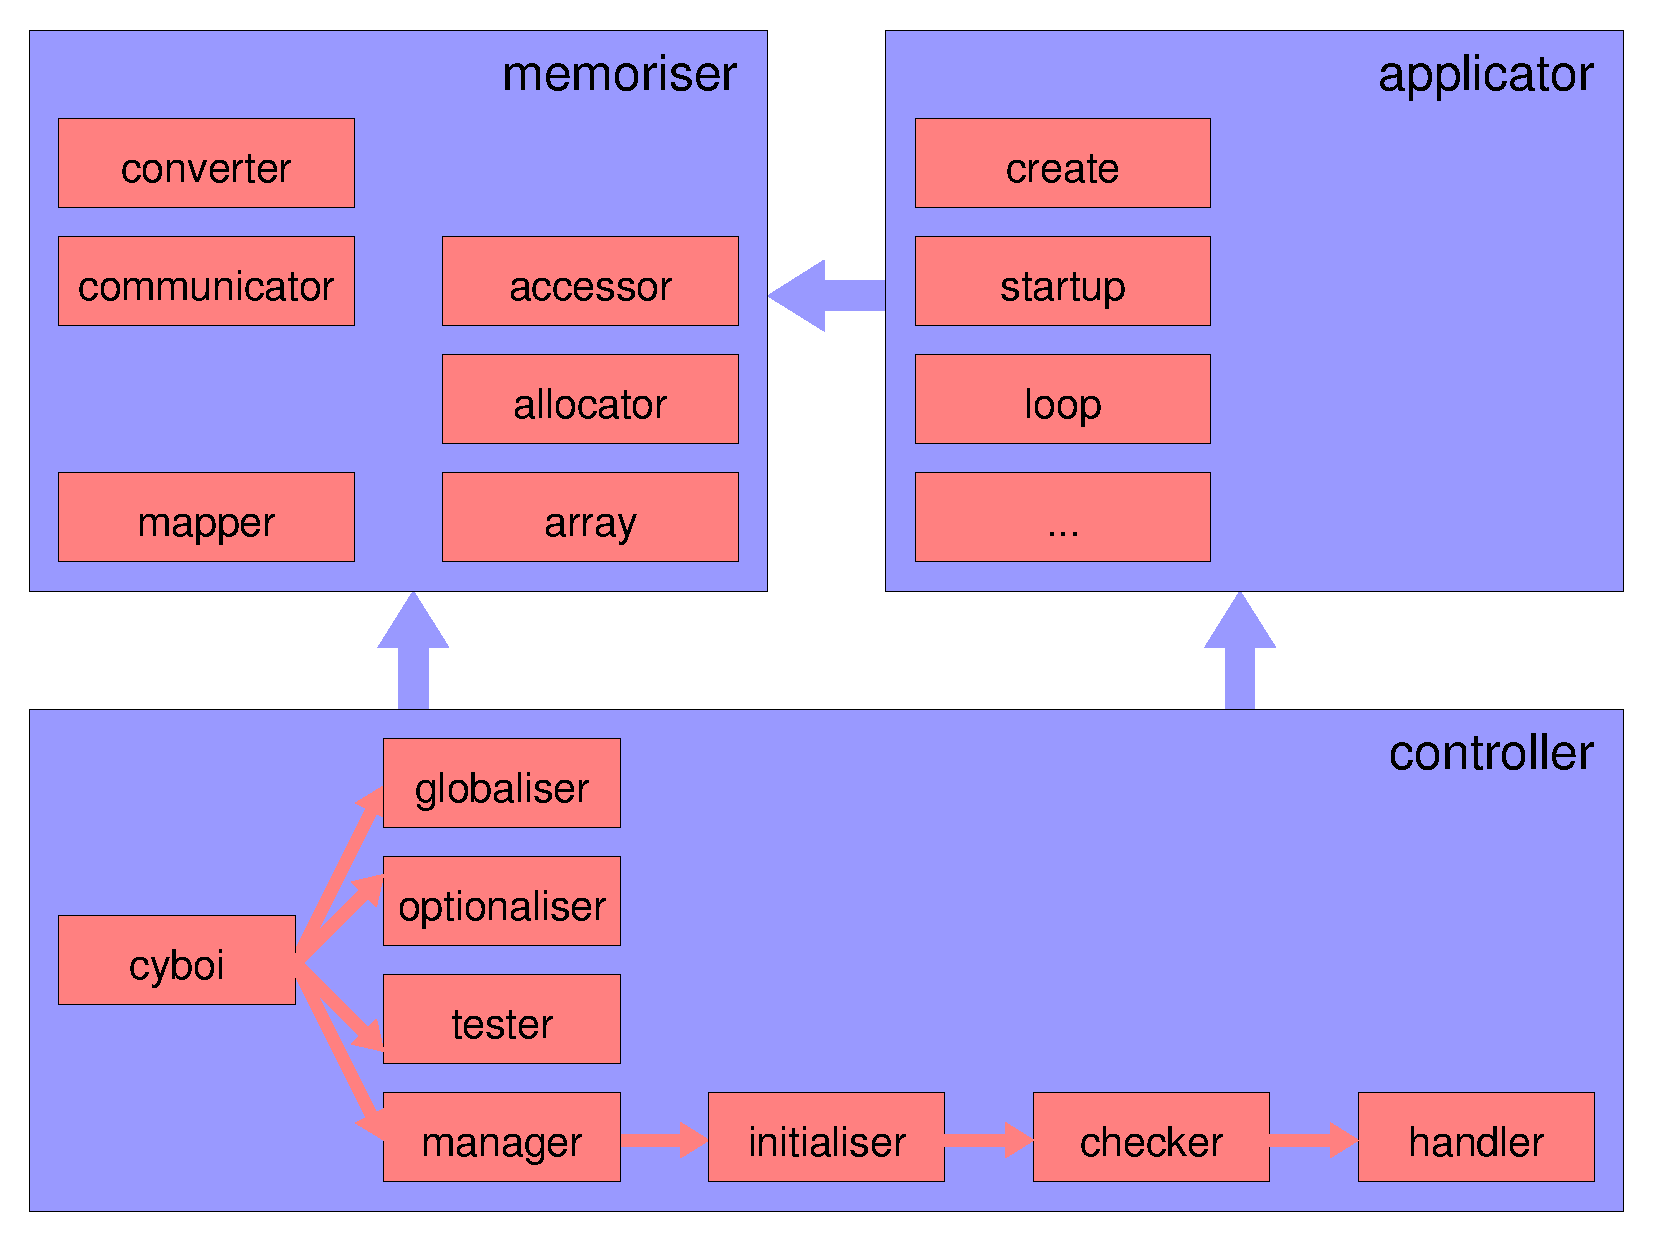
\includegraphics[scale=0.3,angle=-90]{graphic/dependencies.pdf}
        \caption{CYBOI Part Dependencies and Control Flow}
        \label{dependencies_figure}
    \end{center}
\end{figure}

%
% $RCSfile: process_launching.tex,v $
%
% Copyright (C) 2002-2008. Christian Heller.
%
% Permission is granted to copy, distribute and/or modify this document
% under the terms of the GNU Free Documentation License, Version 1.1 or
% any later version published by the Free Software Foundation; with no
% Invariant Sections, with no Front-Cover Texts and with no Back-Cover
% Texts. A copy of the license is included in the section entitled
% "GNU Free Documentation License".
%
% http://www.cybop.net
% - Cybernetics Oriented Programming -
%
% http://www.resmedicinae.org
% - Information in Medicine -
%
% Version: $Revision: 1.1 $ $Date: 2008-08-19 20:41:08 $ $Author: christian $
% Authors: Christian Heller <christian.heller@tuxtax.de>
%

\subsection{Process Launching}
\label{process_launching_heading}
\index{CYBOI Process Launching}
\index{CYBOI main Procedure}

As every other C-, C++- or Java program, CYBOI has a \emph{main} procedure
(\emph{cyboi} module) serving as entry point for its process to run. It
triggers the system lifecycle (in the meaning of startup and shutdown of a
system process). After having initialised global variables and having read the
command line parameter, the rest of the system is started up by the
\emph{manage} procedure (\emph{manager} module).

%
% $RCSfile: lifecycle_management.tex,v $
%
% Copyright (c) 2002-2007. Christian Heller. All rights reserved.
%
% Permission is granted to copy, distribute and/or modify this document
% under the terms of the GNU Free Documentation License, Version 1.1 or
% any later version published by the Free Software Foundation; with no
% Invariant Sections, with no Front-Cover Texts and with no Back-Cover
% Texts. A copy of the license is included in the section entitled
% "GNU Free Documentation License".
%
% http://www.cybop.net
% - Cybernetics Oriented Programming -
%
% Version: $Revision: 1.1 $ $Date: 2007-07-17 20:02:36 $ $Author: christian $
% Authors: Christian Heller <christian.heller@tuxtax.de>
%

\section{Lifecycle Management}
\label{lifecycle_management_heading}
\index{Lifecycle Management}

%
% $RCSfile: startup.tex,v $
%
% Copyright (c) 2002-2007. Christian Heller. All rights reserved.
%
% Permission is granted to copy, distribute and/or modify this document
% under the terms of the GNU Free Documentation License, Version 1.1 or
% any later version published by the Free Software Foundation; with no
% Invariant Sections, with no Front-Cover Texts and with no Back-Cover
% Texts. A copy of the license is included in the section entitled
% "GNU Free Documentation License".
%
% http://www.cybop.net
% - Cybernetics Oriented Programming -
%
% Version: $Revision: 1.1 $ $Date: 2007-07-17 20:02:36 $ $Author: christian $
% Authors: Christian Heller <christian.heller@tuxtax.de>
%

\subsection{Startup}
\label{startup_heading}
\index{Startup}

This operation starts up the given service.

\subsubsection{Service Property}

\emph{required}

name=\texttt{'service'}\\
abstraction=\texttt{'character'}\\
model=\texttt{'signal' \vline\ 'shell' \vline\ 'standard\_output'
    \vline\ 'gnu\_linux\_console' \vline\ 'x\_window\_system' \vline\ 'www' \vline\ 'cyboi'}

This is the service to be started up.

\subsubsection{Namespace Property}

\emph{required}

name=\texttt{'namespace'}\\
abstraction=\texttt{'character'}\\
model=\texttt{'local' \vline\ 'inet' \vline\ 'inet6' \vline\ 'ns' \vline\ 'iso' \vline\ 'ccitt' \vline\ 'implink' \vline\ 'route'}

The namespace of the socket.

\subsubsection{Style Property}

\emph{required}

name=\texttt{'style'}\\
abstraction=\texttt{'character'}\\
model=\texttt{'stream' \vline\ 'datagram' \vline\ 'raw'}

The style of communication.

\subsubsection{Address Property}

\emph{required}

name=\texttt{'address'}\\
abstraction=\texttt{'character'}\\
model=\texttt{'loopback' \vline\ 'any'}

This is the host's address.

%
% $RCSfile: shutdown.tex,v $
%
% Copyright (c) 2002-2007. Christian Heller. All rights reserved.
%
% Permission is granted to copy, distribute and/or modify this document
% under the terms of the GNU Free Documentation License, Version 1.1 or
% any later version published by the Free Software Foundation; with no
% Invariant Sections, with no Front-Cover Texts and with no Back-Cover
% Texts. A copy of the license is included in the section entitled
% "GNU Free Documentation License".
%
% http://www.cybop.net
% - Cybernetics Oriented Programming -
%
% Version: $Revision: 1.2 $ $Date: 2007-08-01 13:59:00 $ $Author: christian $
% Authors: Christian Heller <christian.heller@tuxtax.de>
%

\subsection{Shutdown}
\label{shutdown_heading}
\index{Shutdown}

This operation shuts down the given service.

\subsubsection{Example}

\begin{scriptsize}
    \begin{verbatim}
<part name="shutdown_gui" channel="inline" abstraction="operation" model="shutdown">
    <property name="service" channel="inline" abstraction="character" model="x_window_system"/>
</part>
    \end{verbatim}
\end{scriptsize}

\subsubsection{Service Property}

This is the service to be shut down.

\emph{required}

name=\texttt{'service'}\\
abstraction=\texttt{'character'}\\
model=\texttt{'signal' \vline\ 'shell' \vline\ 'standard\_output'
    \vline\ 'gnu\_linux\_console' \vline\ 'x\_window\_system' \vline\ 'www' \vline\ 'cyboi'}

%
% $RCSfile: exit.tex,v $
%
% Copyright (c) 2002-2007. Christian Heller. All rights reserved.
%
% Permission is granted to copy, distribute and/or modify this document
% under the terms of the GNU Free Documentation License, Version 1.1 or
% any later version published by the Free Software Foundation; with no
% Invariant Sections, with no Front-Cover Texts and with no Back-Cover
% Texts. A copy of the license is included in the section entitled
% "GNU Free Documentation License".
%
% http://www.cybop.net
% - Cybernetics Oriented Programming -
%
% Version: $Revision: 1.2 $ $Date: 2007-08-01 13:59:00 $ $Author: christian $
% Authors: Christian Heller <christian.heller@tuxtax.de>
%

\subsection{Exit}
\label{exit_heading}
\index{Exit}

This operation initiates the shutdown sequence for the application system.

\subsubsection{Example}

\begin{scriptsize}
    \begin{verbatim}
<part name="exit_system" channel="inline" abstraction="operation" model="exit"/>
    \end{verbatim}
\end{scriptsize}


%
% $RCSfile: signal_checking.tex,v $
%
% Copyright (C) 2002-2008. Christian Heller.
%
% Permission is granted to copy, distribute and/or modify this document
% under the terms of the GNU Free Documentation License, Version 1.1 or
% any later version published by the Free Software Foundation; with no
% Invariant Sections, with no Front-Cover Texts and with no Back-Cover
% Texts. A copy of the license is included in the section entitled
% "GNU Free Documentation License".
%
% http://www.cybop.net
% - Cybernetics Oriented Programming -
%
% http://www.resmedicinae.org
% - Information in Medicine -
%
% Version: $Revision: 1.1 $ $Date: 2008-08-19 20:41:08 $ $Author: christian $
% Authors: Christian Heller <christian.heller@tuxtax.de>
%

\subsection{Signal Checking}
\label{signal_checking_heading}
\index{CYBOI Signal Checking}

The \emph{check} procedure consists of an endless loop continuously checking
for signals residing in signal memory. It provides the dynamics and -- so to
say -- keeps the system \emph{alive}. Of all queued signals, the one with
highest priority is retrieved first and forwarded to the \emph{handle}
procedure (\emph{handler} module).

This principle can be observed not only in operating-, but many other kinds of
systems. \emph{Servers} run an endless loop waiting for (network) \emph{Client}
requests. Applications often use signalling mechanisms provided by a framework,
that handles keyboard press- or mouse click signals stemming from a
\emph{Graphical User Interface} (GUI). However, as opposed to the event
handling of such frameworks which relies on bidirectional dependencies since
child components have to register as listener at their parent, a top-level
signal checker loop forwards all events in a unidirectional manner to
interested system parts. It is worth noting that signals may also be produced
internally, as follow-ups, by other signals.

After having been processed, the signal gets removed from the signal memory.
Once an \emph{exit} signal occurs, the shutdown flag is set, so that the signal
checking loop can be left -- and the system be shutdown.

%
% $RCSfile: signal_handling.tex,v $
%
% Copyright (C) 2002-2008. Christian Heller.
%
% Permission is granted to copy, distribute and/or modify this document
% under the terms of the GNU Free Documentation License, Version 1.1 or
% any later version published by the Free Software Foundation; with no
% Invariant Sections, with no Front-Cover Texts and with no Back-Cover
% Texts. A copy of the license is included in the section entitled
% "GNU Free Documentation License".
%
% http://www.cybop.net
% - Cybernetics Oriented Programming -
%
% http://www.resmedicinae.org
% - Information in Medicine -
%
% Version: $Revision: 1.1 $ $Date: 2008-08-19 20:41:08 $ $Author: christian $
% Authors: Christian Heller <christian.heller@tuxtax.de>
%

\subsection{Signal Handling}
\label{signal_handling_heading}
\index{CYBOI Signal Handling}
\index{Central Processing Unit}
\index{CPU}

Depending on the signal model's kind of abstraction, two different signal
handling procedures may be called: \emph{handle\_compound} or
\emph{handle\_operation} (both in the \emph{handler} module). While the former
breaks down composed signals (algorithms) into basic operations, the latter
executes primitive signals (operations) directly, in form of low-level
instructions, which may go down to direct calls of the instruction set of the
\emph{Central Processing Unit} (CPU).

Actual knowledge model changes, in other words the application of well-defined
\emph{Logic-} to \emph{State} models, is done by primitive operations only.

%
% $RCSfile: operation_execution.tex,v $
%
% Copyright (C) 2002-2008. Christian Heller.
%
% Permission is granted to copy, distribute and/or modify this document
% under the terms of the GNU Free Documentation License, Version 1.1 or
% any later version published by the Free Software Foundation; with no
% Invariant Sections, with no Front-Cover Texts and with no Back-Cover
% Texts. A copy of the license is included in the section entitled
% "GNU Free Documentation License".
%
% http://www.cybop.net
% - Cybernetics Oriented Programming -
%
% http://www.resmedicinae.org
% - Information in Medicine -
%
% Version: $Revision: 1.1 $ $Date: 2008-08-19 20:41:08 $ $Author: christian $
% Authors: Christian Heller <christian.heller@tuxtax.de>
%

\subsection{Operation Execution}
\label{operation_execution_heading}
\index{CYBOI Operation Execution}

Each low-level operation has its own module, belonging to the \emph{Applicator}
part of CYBOI. An addition operation is executed in the \emph{add} module, a
comparison operation in the \emph{compare} module, a creation operation in the
\emph{create} module, and so forth. Operations exist for several purposes, some
of which are listed, together with an example operation, following:

\begin{itemize}
    \item[-] program flow (\emph{loop})
    \item[-] boolean logic (\emph{and})
    \item[-] comparison (\emph{equals})
    \item[-] arithmetics (\emph{add})
    \item[-] service control (\emph{startup})
    \item[-] memory management (\emph{create})
\end{itemize}

%
% $RCSfile: model_transition.tex,v $
%
% Copyright (C) 2002-2008. Christian Heller.
%
% Permission is granted to copy, distribute and/or modify this document
% under the terms of the GNU Free Documentation License, Version 1.1 or
% any later version published by the Free Software Foundation; with no
% Invariant Sections, with no Front-Cover Texts and with no Back-Cover
% Texts. A copy of the license is included in the section entitled
% "GNU Free Documentation License".
%
% http://www.cybop.net
% - Cybernetics Oriented Programming -
%
% http://www.resmedicinae.org
% - Information in Medicine -
%
% Version: $Revision: 1.1 $ $Date: 2008-08-19 20:41:07 $ $Author: christian $
% Authors: Christian Heller <christian.heller@tuxtax.de>
%

\subsection{Model Transition}
\label{model_transition_heading}
\index{CYBOI Model Transition}
\index{Knowledge Template}
\index{Knowledge Model}
\index{Information Processing Model}
\index{CYBOI as Universal Data Converter}

The creation of transient knowledge models (to be kept in memory, at runtime)
from persistent knowledge templates (given in form of CYBOL sources) is not a
trivial thing. It is a mechanism consisting of a cascade of model transitions,
comparable to the \emph{Information Processing Model} of cognitive psychology
(section \ref{information_processing_model_heading}). One may imagine this as a
state changing its appearance, while \emph{wandering} through the system. The
same mechanism is applied when handling communication data (figure
\ref{transition_figure}). Because CYBOI's architecture is easily extensible
with various modules, such as \emph{import/ export} (i/e) filters for different
kinds of communication, it may act as universal data converter. All
corresponding modules belong to the \emph{Memoriser} part of CYBOI.

\begin{figure}[ht]
    \begin{center}
        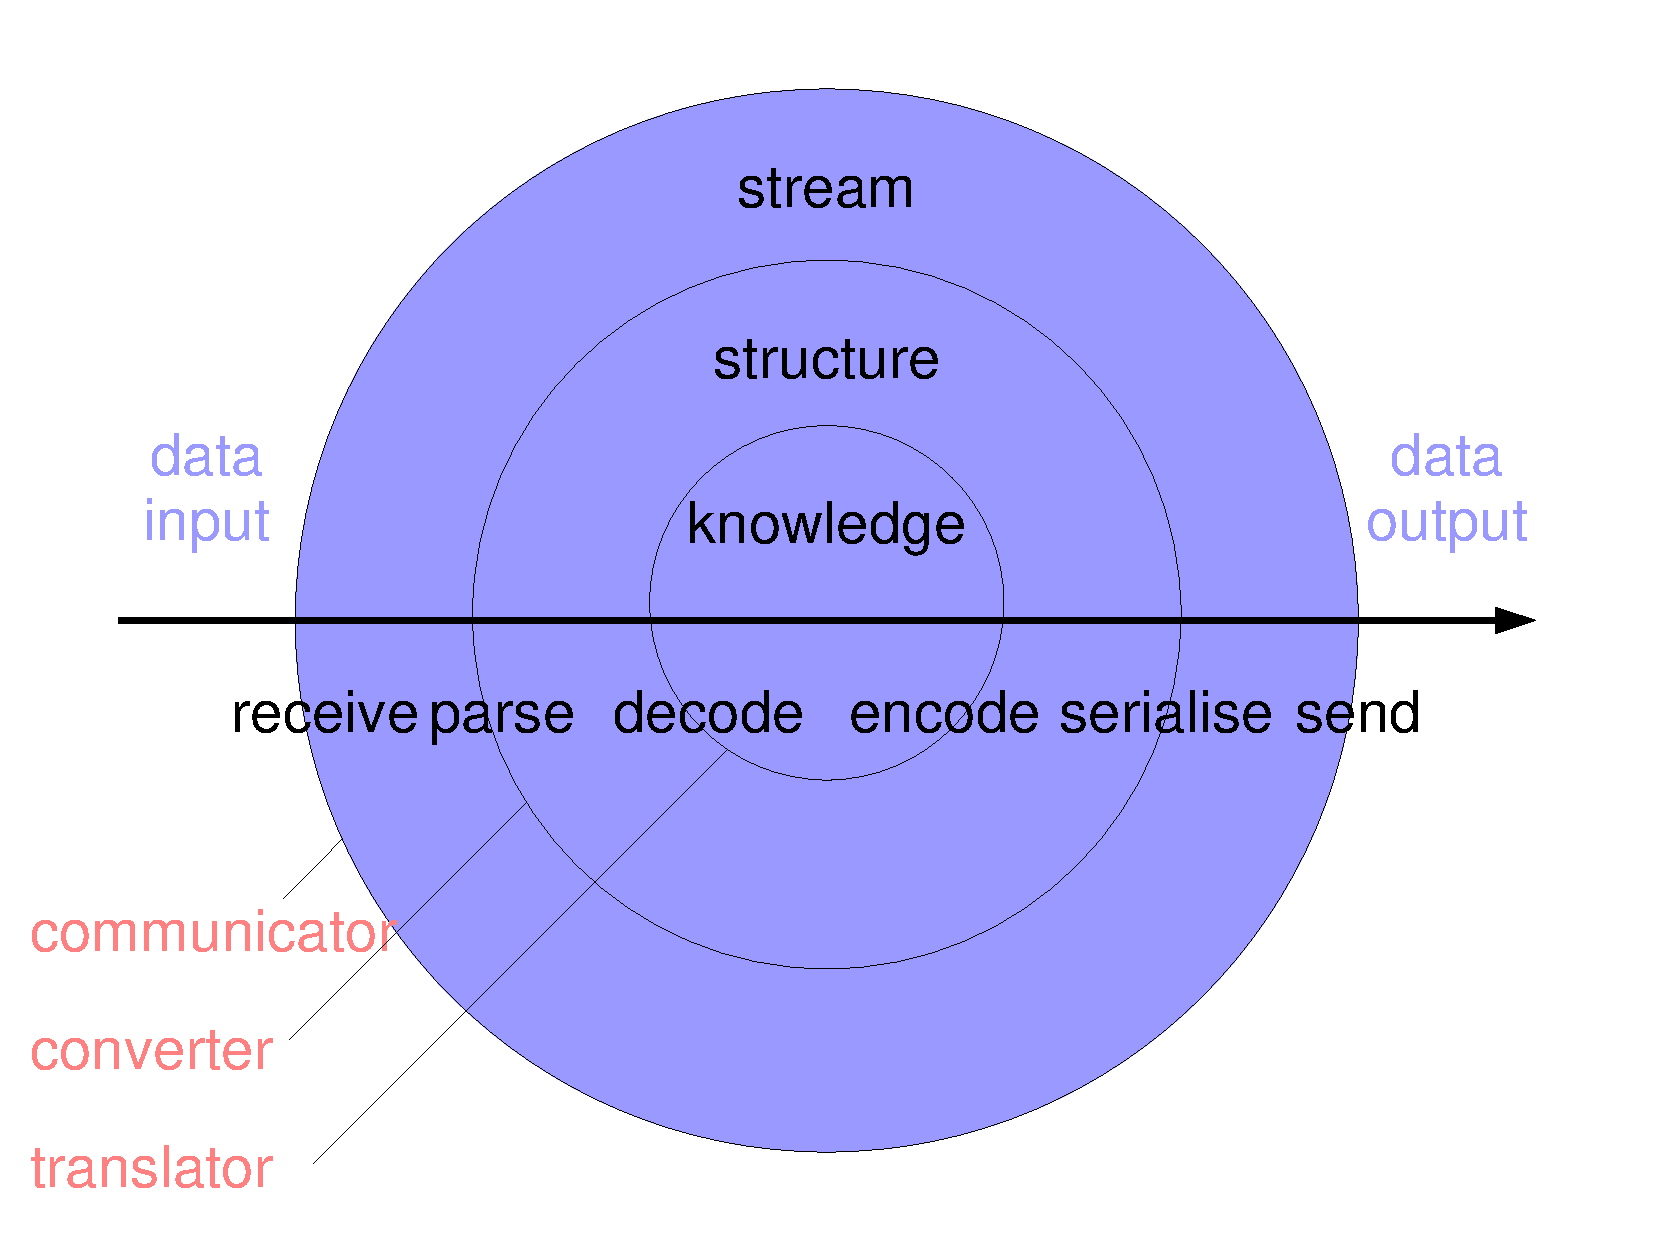
\includegraphics[scale=0.3,angle=-90]{graphic/transition.pdf}
        \caption{Input-to-Output Model Transition}
        \label{transition_figure}
    \end{center}
\end{figure}

As opposed to the knowledge acquirement in \emph{Artificial Neural Networks}
(ANN),
%(section \ref{artificial_neural_network_heading}),
the knowledge in CYBOP
systems is not learned, but \emph{injected} by reading from external knowledge
sources, which can be manipulated in a flexible manner any time. The difference
to standard applications is that these hard-wire their knowledge within the
system.

A data input (i/p), after having been processed by a \emph{receive} procedure
(\emph{communicator} modules), results in a stream -- a data array in memory. A
\emph{parse} procedure (\emph{converter} modules), depending on the kind of
abstraction of the data, then builds a structure out of this simple array. The
structure, finally, passes a \emph{decode} procedure (\emph{translator}
modules) which creates a knowledge model.

Whenever an application running within CYBOI wants to send data, may it be to
another system or for making them persistent on a local \emph{Hard Disk Drive}
(HDD), translator, converter and communicator have to be crossed in the
opposite direction. Because a running application system is a tree of knowledge
models allocating space in memory, parts of that tree can be \emph{serialised}
easily. It has to be mentioned, though, that slight changes of the XML format
are necessary to achieve this: The usual quotation marks used to delimit XML
attribute values have to be replaced with differing \emph{begin} and \emph{end}
characters. This feature is an open issue which the current version of CYBOI
does not provide yet.

%Isn't CYBOI model transition similar to termios Zeichenverarbeitung in Linux?
%siehe Grafik im Buch: Anwendungen entwickeln unter Linux, S. 249

%
% $RCSfile: data_creation.tex,v $
%
% Copyright (C) 2002-2008. Christian Heller.
%
% Permission is granted to copy, distribute and/or modify this document
% under the terms of the GNU Free Documentation License, Version 1.1 or
% any later version published by the Free Software Foundation; with no
% Invariant Sections, with no Front-Cover Texts and with no Back-Cover
% Texts. A copy of the license is included in the section entitled
% "GNU Free Documentation License".
%
% http://www.cybop.net
% - Cybernetics Oriented Programming -
%
% http://www.resmedicinae.org
% - Information in Medicine -
%
% Version: $Revision: 1.1 $ $Date: 2008-08-19 20:41:06 $ $Author: christian $
% Authors: Christian Heller <christian.heller@tuxtax.de>
%

\subsection{Data Creation}
\label{data_creation_heading}
\index{CYBOI Data Creation}
\index{CYBOI Data Encapsulation}
\index{Compound Structure as Multi Dimensional Container}
\index{Knowledge Memory consisting of Compound- and Primitive Models}

The functionality of CYBOI as system is built around the manipulation of states
in memory. The question how states, representing data, are stored is therefore
of great importance. Besides containers like the \emph{Internals Memory},
\emph{Knowledge Memory} and \emph{Signal Memory}, belonging to its
infrastructure, CYBOI uses special structures encapsulating primitive data. Not
only types like \emph{Character}, \emph{Integer}, \emph{Float} or \emph{String}
are wrapped this way, also \emph{Operations} are. Any compositions of these are
stored as \emph{Compound}.

Encapsulated primitives have the advantage of being forwardable as reference
(memory address pointer), instead of as copy. This ensures that redundant data
are avoided and states of manipulated primitives are not lost. \emph{Logic}
operations are stored in form of a string indicating their name. Necessary
references to input/ output (i/o) \emph{State} models need to be provided as
meta information, by the compound model surrounding the operation.

The \emph{Compound}, as most important CYBOI structure capable of representing
state- as well as logic knowledge, and capable of emulating a map, collection,
list and tree, deserves closer inspection. Essentially, it is a container able
to recursively reference instances of its own, thus spanning up a tree of parent
nodes (\emph{Whole} models) that may have child nodes (\emph{Part} models). In
fulfillment of the requirements of the knowledge schema introduced in section
\ref{knowledge_representation_heading}, a compound consists of a combination of
many arrays containing a part's:

\begin{itemize}
    \item[-] \emph{Name:} serving as unique \emph{Identifier} (ID)
    \item[-] \emph{Model:} the actual contents (may be a part node)
    \item[-] \emph{Abstraction:} the kind of abstraction (type) of the model
    \item[-] \emph{Details:} further meta information (properties, constraints)
\end{itemize}

One may call the \emph{Compound} a \emph{multi-dimensional} container but it is
probably easier described as large table with many columns, whereby the values
of one row describe exactly one part model, and thus belong together.

The previously mentioned \emph{Knowledge Memory} may be seen as huge tree
consisting of compound- as well as primitive models. Its root is always a
\emph{Compound} -- it, so to say, concentrates all knowledge in just one point,
the single concepts being branches of it.

The essential procedures for managing data in memory are \emph{create} and
\emph{destroy} (\emph{creator} modules). Three additional kinds of procedures
are provided for compound- and other container-like structures: \emph{set},
\emph{get} and \emph{remove} (\emph{accessor} modules). It should be noted at
this point that CYBOL applications have no direct access to these procedures,
so that \emph{wild} memory allocation is not possible. A knowledge model can
only be created using the corresponding CYBOL operation \emph{create\_part}.

%%
% $RCSfile: instance.tex,v $
%
% Copyright (C) 2002-2008. Christian Heller.
%
% Permission is granted to copy, distribute and/or modify this document
% under the terms of the GNU Free Documentation License, Version 1.1 or
% any later version published by the Free Software Foundation; with no
% Invariant Sections, with no Front-Cover Texts and with no Back-Cover
% Texts. A copy of the license is included in the section entitled
% "GNU Free Documentation License".
%
% http://www.cybop.net
% - Cybernetics Oriented Programming -
%
% http://www.resmedicinae.org
% - Information in Medicine -
%
% Version: $Revision: 1.1 $ $Date: 2008-08-19 20:41:07 $ $Author: christian $
% Authors: Christian Heller <christian.heller@tuxtax.de>
%

\subsection{Instance}
\label{instance_heading}

CYBOI Translator for model creation is NOT the same as a CYBOL translator model!

- while knowledge in a system exists as huge (transient) hierarchy,
it is defined in discrete (persistent) templates outside
- processing of source code (knowledge templates):
1 persistent model
2 transient received/read model
3 parsed model
4 decoded model

Application knowledge is kept in form of \emph{Templates} of which \emph{Instances}
can be created. Knowledge instances are \emph{Clones} (section \ref{clone_heading}).
Every knowledge instance can become a template itself.

While a knowledge instance is stored as one huge, serialisable tree in memory,
its template is split up into smaller, inter-related concepts. This technique
is known from \emph{Object Oriented Programming} (OOP) (section
\ref{object_oriented_programming_heading}) where knowledge templates are called
\emph{Class}. It was introduced to increase the reuse of existing knowledge
models, avoiding redundant implementations.

\begin{figure}[ht]
    \begin{center}
        \includegraphics[scale=0.3,angle=-90]{graphic/instantiation.pdf}
        \caption{Knowledge Template Instantiation (Creation and Destruction)}
        \label{instantiation_figure}
    \end{center}
\end{figure}

